\section{Data Governance} \label{section: DATAG}

Data Governance, is the organizing framework that establishes internal data policies that apply to how data is gathered, stored, processed. 

In the context of designing an infrastructure with SAS technologies, UHTASI assumes the responsibility of establishing data governance policies that adhere to HIPAA compliance standards, standardized security practices, and industry best-practices of sharing data. This obligation arises from the overarching goal of MLA, which is to provide data analytic services for PHI data.

Note that this chapter does not aim to be a comprehensive handbook for the implementation of proper data governance but offers an overview of data governance methodologies. Information was gathered from the SAS conference on data governance (May, 2023).

\subsection{SAS Data Management Framework}
The SAS Data Management Framework is a collection of groups and methodologies that offer solutions for data integration, data quality, data governance, and metadata management. 

\begin{figure}[H]
\begin{center}
    \renewcommand{\arraystretch}{1.5}
    \begin{tabular}{|>{\raggedright\arraybackslash}m{3.5cm}
                    |>{\raggedright\arraybackslash}m{11.5cm}
                    |}
    \hline
    \rowcolor[HTML]{196fb4}\centering\textcolor{white}{\large Principle} 
                            & \centering\textcolor{white}{\large Description} 
                            \tabularnewline 
    \hline
    Program Objectives & The, "why?", establishes the goals and purpose of the data governance program. \\\hline
    Guiding Principles & The, "how?, outlines the framework for making data-related decisions and ensuring consistency and alignment with organizational goals and values. \\\hline
    Decision-making Bodies & The, "who?", identifies the decision-making bodies or committees responsible for overseeing and making key data governance decisions, ensuring representation from relevant experts. \\\hline
    Decision Rights & The, "what?", allocates decision-making authority and responsibilities to clarify accountability and effective data management and control. \\\hline
    \end{tabular}
\end{center}
\caption{4 Principles of Data Governance}
\label{4 DG Principles}
\end{figure}

\begin{figure}[H]
    \centering
    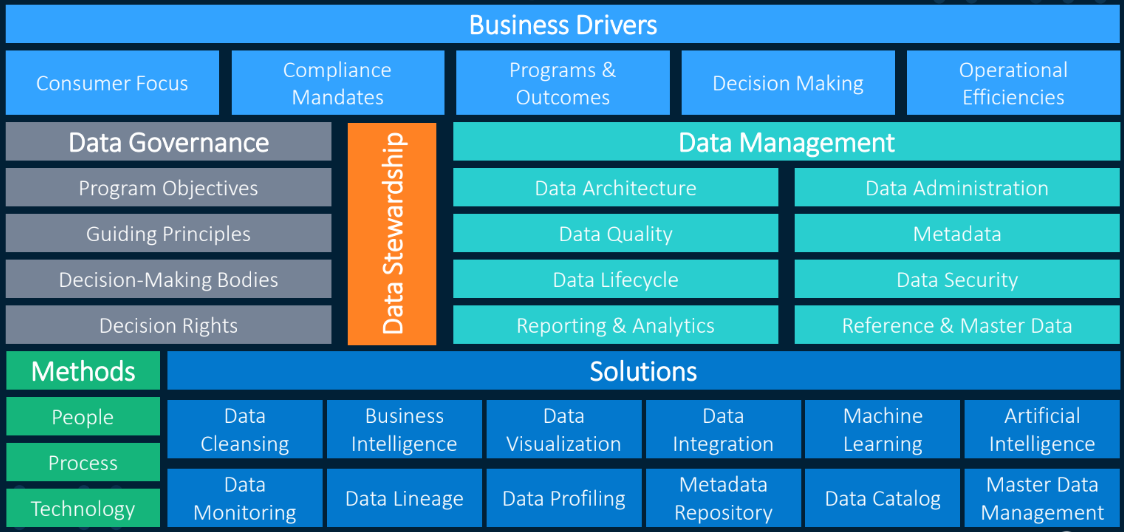
\includegraphics[scale=0.55]{images/SAS Data Management Framework.png}
    \caption{SAS Data Management Framework}
    \label{SAS DMF}
\end{figure}

SAS Data Management, as part of the SAS Data Management Framework, is a set of principles that cover policies and standards about data collection, storage, and processes. 

\begin{figure}[H]
\begin{center}
    \renewcommand{\arraystretch}{1.5}
    \begin{tabular}{|>{\raggedright\arraybackslash}m{3.5cm}
                    |>{\raggedright\arraybackslash}m{11.5cm}
                    |}
    \hline
    \rowcolor[HTML]{196fb4}\centering\textcolor{white}{\large Principle} 
                            & \centering\textcolor{white}{\large Description} 
                            \tabularnewline 
    \hline
    Data Architecture & Models, policies, rules, standards about what data is captured, how it is stored, arranged and integrated (data analysis, data modeling, data design). \\\hline
    Data Quality & Quality of data, its integrity and how its is cleansed and/or enriched. \\\hline
    Data Lifecycle & How data is created, stored, distributed, used, maintained, archived, and disposed. \\\hline
    Reporting & Analytics \& Systems that support the creation of value from data. \\\hline
    Data Administration & Day-to-day management and control of data and databases. \\\hline
    Metadata & Capture, storage, documentation, and publishing of information about enterprise data such as its description, lineage, usage, ownership, etc. \\\hline
    Data Security & How data is accessed and secured and how privacy is handled. \\\hline
    Reference \& Master Data & Correct and consistent management of master and reference data. \\\hline
    \end{tabular}
\end{center}
\caption{8 Principles of Data Management}
\label{8 DMA Principles}
\end{figure}

\begin{figure}[H]
    \centering
    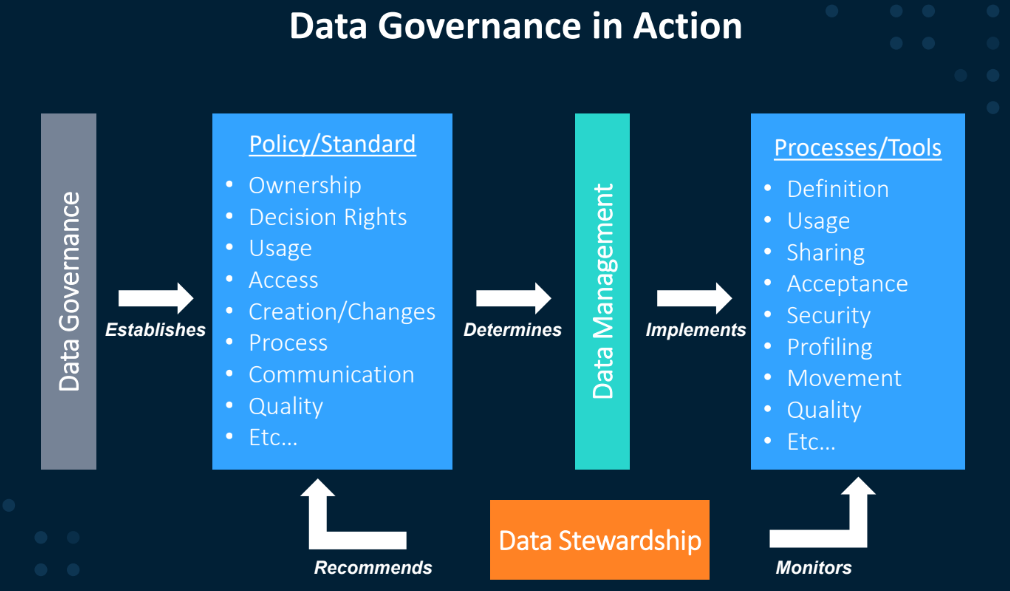
\includegraphics[scale=.60]{images/SAS Data Governance In Action.png}
    \caption{SAS Data Governance in Action}
    \label{SAS DGIA}
\end{figure}

Engaging in data governance without achieving data management outcomes is merely an academic exercise and is bound to fail. Similarly, conducting data management without proper data governance perpetuates a culture of reliance on unreliable sources and informal knowledge sharing. 

Data stewards play a vital role in actively monitoring data and advocating for organizational policies, serving as the vital link between data governance and data management activities.

\subsection{Data Stewardship}
A data steward is someone whose role is to develop and protect the information resources for the organization and ensures the integrity of the data. However, data stewardship is not data governance, it is a critical part of data governance. 

\begin{figure}[H]
\begin{center}
    \renewcommand{\arraystretch}{1.5}
    \begin{tabular}{|>{\raggedright\arraybackslash}m{4cm}
                    |>{\raggedright\arraybackslash}m{8cm}
                    |}
    \hline
    \rowcolor[HTML]{196fb4}\centering\textcolor{white}{\large Principle} 
                            & \centering\textcolor{white}{\large Description} 
                            \tabularnewline 
    \hline
    Metadata & Common definitions, Data dictionary, Data mining, Data lineage. \\\hline
    Data Quality & Continuous improvement, Root cause analysis, Measurement. \\\hline
    Architecture & Standards, Scalable solution(s). \\\hline
    Data Trust & Standards, Policies. \\\hline
    Data Integration & Transparent processes, Data ready for use. \\\hline
    People and Process & Teamwork, Facilitation, Consensus building. \\\hline
    Business Needs & Identify, Set priorities, Alignment of data with business needs. \\\hline
    Communication & Catalyst for change, Data evangelist.\\\hline
    \end{tabular}
\end{center}
\caption{8 Principles of Data Stewardship}
\label{Data Steward's Job}
\end{figure}

\subsection{Metadata}
Metadata can be defined as data about data, serving as valuable information that assists in navigating the intricate network of data within an organization and facilitates its effective utilization.

\subsubsection{Metadata Management}
The practice of gathering, storing, and provisioning information about data assets.

Metadata plays a crucial role in various aspects of data management and analytics within an organization. It serves to increase confidence in the data by providing valuable context and understanding. 

Operational efficiencies are harmonized as redundant data and processes are identified, streamlining operations. Effective communication between data creators, consumers, and IT is facilitated, fostering collaboration and alignment. This reduces the time to market by decreasing the development life cycle and enabling faster data research. Change management and impact analysis for IT become simpler, ensuring smooth transitions and minimizing disruptions. 

\subsubsection{Types of Metadata}
There are 3 types of metadata used by organizations.

\begin{figure}[H]
\begin{center}
    \renewcommand{\arraystretch}{1.5}
    \begin{tabular}{|>{\raggedright\arraybackslash}m{3.5cm}
                    |>{\raggedright\arraybackslash}m{3cm}
                    |>{\raggedright\arraybackslash}m{8cm}
                    |}
    \hline
    \rowcolor[HTML]{196fb4}\centering\textcolor{white}{\large Metadata Type} 
                            & \centering\textcolor{white}{\large Data Owner} 
                            & \centering\textcolor{white}{\large Metadata Objective} 
                            \tabularnewline 
    \hline
    Business Metadata & Business & Provide a road map to navigate in business context the complex network of data an organization has. \\\hline
    Technical Metadata & Technical & Technical characteristics of data used by IT staff to design efficient databases, queries, and applications and to reduce data duplication.\\\hline
    Operational Metadata & Technical & Describes characteristics of routine operations.\\\hline
    \end{tabular}
\end{center}
\caption{Types of Metadata}
\label{Types of Metadata}
\end{figure}

\begin{enumerate}
    \item Business Metadata Examples:
    \begin{itemize}
        \item Business name and description, data location, data usage, business rules, access instructions, valid range of values, relationship to other data elements, data owner and steward, and data security classification.
    \end{itemize}
    \item Technical Metadata Examples: 
    \begin{itemize}
        \item Table name, column name, data type, data size, primary and foreign key attributes, optionality, nullability, database server identifier, and data lineage.
    \end{itemize}
    \item Operational Metadata Examples:
    \begin{itemize}
        \item Schedules and batch jobs, logs of job execution, error logs, audit, balance, and control measures, SLA requirements, volume and usage statistics, backup and archival information, and daily ETL processes.
    \end{itemize}
\end{enumerate}

\begin{figure}[H]
    \centering
    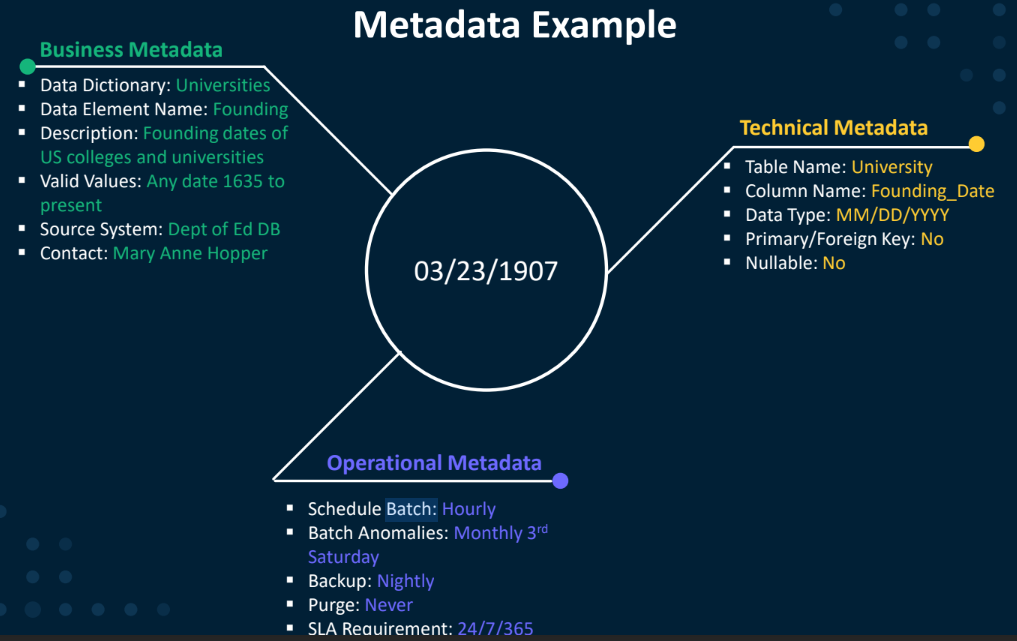
\includegraphics[scale=0.60]{images/Metadata Example.png}
    \caption{Example of Metadata}
    \label{Metadata Example}
\end{figure}

\subsubsection{Metadata Management Cycle}

\begin{figure}[H]
    \centering
    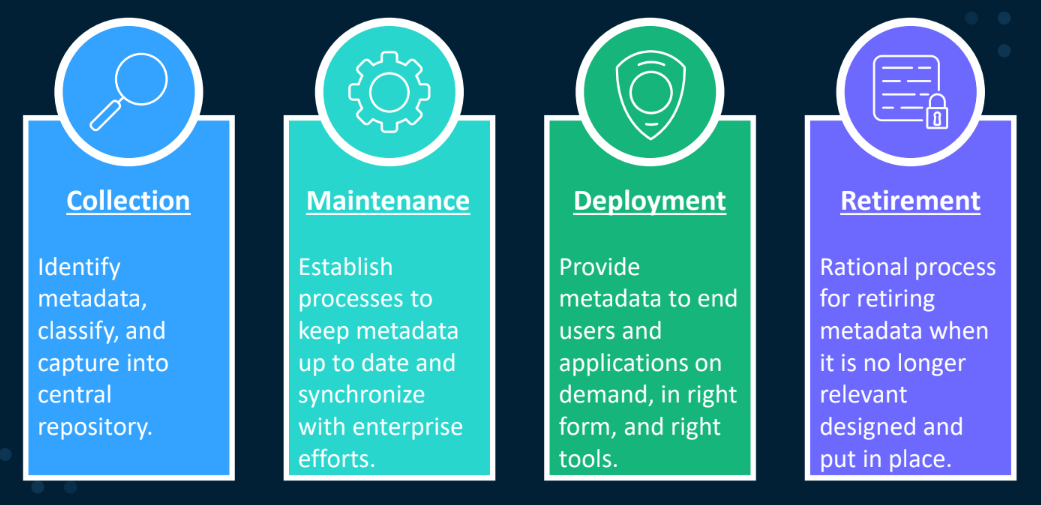
\includegraphics[scale=0.58]{images/Metadata Management Lifecycle.png}
    \caption{Metadata Management Lifecycle}
    \label{Metadata Management Lifecycle}
\end{figure}

\subsection{Data Dictionaries}
A data dictionary defines the structure and contents of data sets, databases, applications, or warehouses.

A recommended approach involves using a standardized document to create a proper dictionary that provides insights into the structure and contents of data sets, databases, applications, or warehouses. Developing a data dictionary requires access to the data, which may necessitate data sharing agreements such as business association agreements for HIPAA compliance. The data dictionary acts as a reference guide that defines the various aspects of data, aiding in its management and utilization. 

To begin building a data dictionary, it is recommended to start with organization critical metadata elements. 

\begin{figure}[H]
\begin{center}
    \renewcommand{\arraystretch}{1.5}
    \begin{tabular}{|>{\raggedright\arraybackslash}m{3.5cm}
                    |>{\raggedright\arraybackslash}m{11cm}
                    |}
    \hline
    \rowcolor[HTML]{196fb4}\centering\textcolor{white}{\large Data Dictionary} 
                            & \centering\textcolor{white}{\large Description}
                            \tabularnewline 
    \hline
    Data Element Name & Business name of element \\\hline
    Description & Business Description \\\hline
    Data Type & Physical data type (varies depending on database platform) \\\hline
    Valid Values & Valid data ranges; 1,0 for measures; valid date range \\\hline
    Source System & Source system database - may need to insert additional columns for multiple load stops (staging, DW $\rightarrow$ DM) \\\hline
    Contact & Data Owner or Data Steward contact person \\\hline
    \end{tabular}
\end{center}
\caption{Key Organization Critical Metadata Elements}
\label{Data Dictionary}
\end{figure}

%<---------------- second day ---------------->
\subsection{Data Quality}
Data quality is the conformance of data to the business definitions and the business rules (i.e., business metadata).

\subsubsection{Data as a True Asset}
Effective planning and management of data is essential, as it is a valuable and reusable asset that can increase in value through integration and analysis. Managing the quality of both data and metadata is crucial, requiring input from cross-functional teams with diverse skills and expertise. 

Data possesses unique properties, and its value can be expressed both qualitatively and quantitatively. Taking an enterprise-wide perspective is necessary to fully leverage the potential of data and maximize its value.

\subsubsection{Organizational Reasons for Poor Data Quality}
The lack of data stewardship and data governance, along with poor metadata management and absence of data lineage, contribute to misconceptions about data quality. 

Key data elements may not be clearly defined, and the emergence of new data sources outpaces effective management. Manual data entry without quality checks further hampers data integrity. Insufficient monitoring, reporting, and absence of defined service level agreements for essential business data quality exacerbate the issue. Moreover, the absence of clear data ownership and a culture that recognizes data as a valuable business asset perpetuate these data quality misconceptions.

\subsubsection{Data Quality Scope}
\begin{itemize}
    \item Business Definition Quality (\textit{Context})
    \begin{itemize}
        \item Business Definitions. Business Rules. Valid Content (valid values, range). Intended Business Purpose (correct usage context). Current Data Quality.
    \end{itemize}
    \item Data Record Quality (\textit{Rows})
    \begin{itemize}
        \item Item completion. Duplication. Cross-table validation. Accuracy.
    \end{itemize}
        \item Data Element Quality (\textit{Columns})
    \begin{itemize}
        \item Domain Integrity: Data type of field (ex. Date). Correct Contextual Value: Business metadata and business rule validation. Accuracy: Source system or expected calculation validation. Cross-Field Validation: Validates the business rule that relates two or more
        columns or across tables. Format Consistency: Correct format (ex. MM/DD/YYYY).
    \end{itemize}
    \item Data Movement Quality (\textit{Navigation})
    \begin{itemize}
        \item External data quality (incoming – outgoing). Source System to Source System (file transfer, SOA). Source System to data mart / data warehouse. Data Warehouse to Data Marts. To desktops via self-service data. Internal to Cloud – Cloud to Internal. 
    \end{itemize}
\end{itemize}

\subsection{Data Governance Journey}

\subsubsection{Plan: Identify organization needs, opportunities, and efforts}
During the planning phase, objectives of the program must be defined and frameworks must be set for how and when decisions will be made.

The planning phase must discuss the initial scope of data governance, objectives, guiding principles, organizational frameworks, roles, responsibilities, and the program charter.  

\subsubsection{Design: Who makes the decisions and how}
During the design phase, decision-making bodies will determine operating procedures and how
compliance and progress will be measured. Design methodologies should be decided by an official council of data stewards. 

A defined subset of rules should be established that are non-negotiable and must be strictly adhered to. The success of these rules lies in their ability to facilitate the progress of data stewardship, thereby generating tangible value. To validate the effectiveness of your plan, it is recommended to develop a program measurement plan.

This plan involves comparing the current state with previous meetings, using metrics such as steward attendance. For instance, evaluating decision-making based on a required quorum, such as 8 out of 10 members, ensures a robust decision-making process. Furthermore, it is important to note that proxies are not permissible, and the punctuality of members attending the meetings should also be monitored as part of the measurement plan.

A standardized solution to define key activities and assign decision making rights is through a RACI chart. 

\begin{figure}[H]
    \centering
    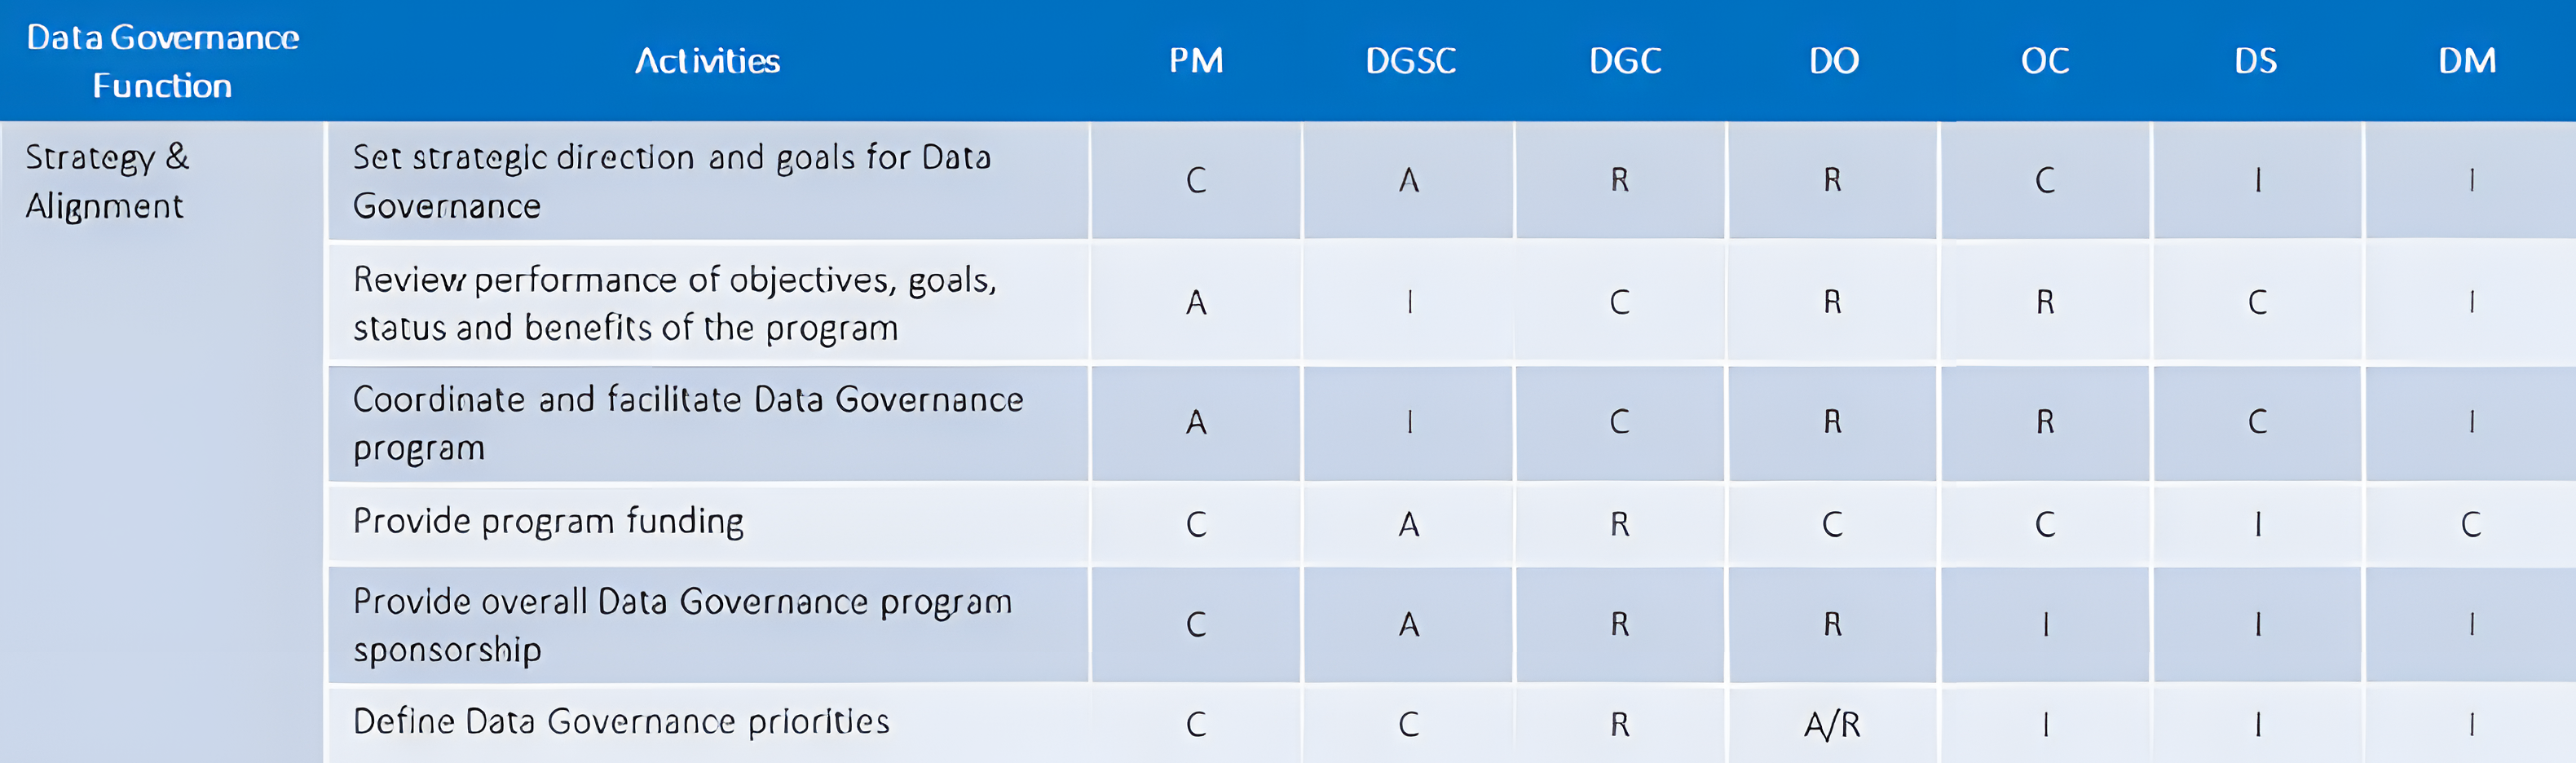
\includegraphics[scale=0.143]{images/RACI-example.png}
    \caption{A Sample RACI Chart \\ \textit{R} = Responsible, \textit{A} = Accountable, \textit{C} = Consulted, \textit{I} = Informed}
    \label{RACI-example}
\end{figure}

\subsubsection{Launch: Kick off initial program – begin small and expand}
During the launch phase, the designed operating model will be executed. 

\begin{enumerate}
    \item Onboard participants: Engage and onboard relevant stakeholders, ensuring their understanding of their roles and responsibilities within the project.
    \item Execute operating model: Implement the established operating model, which defines the framework and processes for data governance.
    \item Policy development and approval: Develop and finalize data governance policies, ensuring alignment with organizational objectives and obtaining necessary approvals.
    \item Benefit measurement: Establish a measurement plan to assess the effectiveness of the data governance. This involves defining metrics and tracking progress against predefined goals.
\end{enumerate}

\subsection{Policy}
A policy refers to a documented set of principles, guidelines, and rules that govern the management, access, usage, and protection of data within an organization. 

\begin{figure}[H]
\begin{center}
    \renewcommand{\arraystretch}{1.5}
    \begin{tabular}{|>{\raggedright\arraybackslash}m{3cm}
                    |>{\raggedright\arraybackslash}m{11.5cm}
                    |}
    \hline
    \rowcolor[HTML]{196fb4}\centering\textcolor{white}{\large Principle} 
                            & \centering\textcolor{white}{\large Description}
                            \tabularnewline 
    \hline
    Policy & Formal set of statements that define how data resources will be used or managed. \\\hline
    Procedure & Detailed instructions about how a policy is to be implemented.\\\hline
    Standard & Required configuration that is considered best practice. \\\hline
    Best Practice & Technique, method, process, or activity that is more effective at delivering a particular outcome than any other technique, method, process, etc. \\\hline
    Data Management & Tactical execution and enforcement of data governance policies and standards. \\\hline
    \end{tabular}
\end{center}
\caption{Principle Comparison Against Policy}
\label{Policy Comparison}
\end{figure}

\subsubsection{Policy Statement - Sample}
The Data Governance Office, in partnership with the appropriate organization entities and support from IT, will proactively assess, monitor, report, and improve data quality. For the purposes of this policy, data quality is defined as the conformance of data to the definitions and the organization rules (metadata).

\subsection{Additional: Questions \& Answers}

To ensure the conversation remains as relevant as possible to UHTASI, dedicated time slots were allocated for question and answer sessions. (Key: \textit{UHTS = UHTASI, SAS = SAS})

\begin{enumerate}
    \item UHTS $\rightarrow$ SAS: \textit{Is there a formal data strategy that outlines, access, integration, movement, storage?}
    \begin{itemize}
        \item \textit{The inherent issue is that not everything is harmonized across organizations, therefore, there is no unified organizational strategy that solves the problem. Instead, the one responsible for providing a solution that fits the organizational needs is the principle investigator.}
    \end{itemize}
    \item SAS $\rightarrow$ UHTS: \textit{How does UHTASI handle data validation?}
    \begin{itemize}
        \item UHTASI mainly uses hash check-sums in R and python for data validation. We hope that SAS software alleviate these, or lack-there-of, validation issues. UHTASI checks for missing cells and duplicates in data, however, these cases do not entirely indicate missing data values. Data sources are not standardized amongst our data providers. Therefore, ETL pipelines, data integration, and data quality are also not standardized.
    \end{itemize}
    \item SAS $\rightarrow$ UHTS: \textit{What are common problems that UHTASI's analysts are facing regarding data?}
    \begin{itemize}
        \item UHTASI's ETL process is dependent on the type of data source that is being used. In the case of federal government data, UHTASI will be provided be an encrypted drive with public/private key authentication processes. However, even a straight forward solution as above requires the tracking an auditing of actions throughout the ETL process. 
        \item UHTASI has difficulty getting access to timely data. Data is provided quarterly by vendors and general trust are established across each vendor.
    \end{itemize}
\end{enumerate}

% < ------- third day ----------->
\newpage
%What are we installing?
\begin{itemize}
    \item SAS 9
    \begin{itemize}
        \item Base SAS
        \item Data Management Advanced Server
        \begin{itemize}
            \item Data Governance - DG Lineage, DDG Workflow, 
            \item Data Integration Studio - High/Enterprise level data access, integration, and management using visual flow charts. (Flow charts are converted to SAS code). More for IT/Admin.
            \item Data Quality - Helps standardize data, duplicate records, errors using visual flow charts and built in (out-of-box) algorithms. (Flow charts are converted to SAS code). More for "everybody". Meant to integrate with other software smoothly because data quality should be checked throughout the entire ETL process. 
            \item Enterprise Guide - Low/Mid data management and access using visual flow charts. (Flow charts are converted to SAS code). More for "everybody".
        \end{itemize}
        \item SAS/ACCESS to MS
    \end{itemize}
    \item SAS Viya
    \begin{itemize}
        \item Viya Platform
        \item Visual Analytics
        \item Visual Statistics
        \item Visual Data Mining and ML
        \item Visual Text Analytics
        \item Visual Forecasting
        \item Model Manager
        % Software below will not be covered but is installed.
        \item SAS Optimization
        \item SAS IML
        \item SAS QC
        \item SAS Econometrics
        \item Data Preparation 
        \item SAS/ACCESS Engines
        \item Visual Analytics Add-In For Office 
    \end{itemize}
\end{itemize}

% <------------ additional questions ----------->